\documentclass[11pt]{article}
\usepackage[margin=1in]{geometry}
\usepackage{tikz}
\usepackage{array}
\usepackage{amsmath}
\begin{document}
\section*{Simply supported beam with a uniform distributed load}
The beam is simply supported at both ends. The uniform load $q=-1000$ N/m is represented by equivalent nodal forces and end moments on a 10 element mesh. The material and section data are $E=2.0690e+11$ Pa, $\nu=0.29$, $G=8.0194e+10$ Pa, $I_z=1$ m$^4$, $J=1$ m$^4$, and $L=10$ m.

\subsection*{Configuration}
\begin{center}
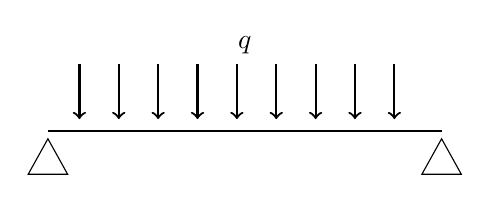
\begin{tikzpicture}[scale=1.0]
\draw[thick] (0,0)--(5,0);\draw (0,-0.1)--(-0.25,-0.55)--(0.25,-0.55)--cycle;\draw (5,-0.1)--(4.75,-0.55)--(5.25,-0.55)--cycle;\foreach \x in {0.4,0.9,...,4.6}{\draw[->,thick] (\x,0.85)--(\x,0.15);}\node[above] at (2.5,0.85) {$q$};
\end{tikzpicture}
\end{center}

\subsection*{Analytical Reference}
$v(L/2)=5qL^4/(384EI_z)$ and $\theta_z(0)=qL^3/(24EI_z)$.

\subsection*{Numerical Comparison}
\begin{center}
\begin{tabular}{|>{\raggedright\arraybackslash}p{0.18\linewidth}|r|r|r|r|r|}
\hline
Quantity & Analytical & C++ & Python & Python vs. analytical & Python vs. C++ \\
\hline
$v_y(L/2)$ & -6.29329789e-07 & -6.29329800e-07 & -6.29329800e-07 & 1.756e-06\% & 0.000e+00\% \\
$\theta_z(0)$ & -2.01385532e-07 & -2.01385530e-07 & -2.01385530e-07 & 1.223e-06\% & 0.000e+00\% \\
\hline
\end{tabular}
\end{center}

\subsection*{Evaluation}
The Python and C++ results are numerically identical to the precision written in the VTK files for the selected critical quantities. The remaining discrepancy with the analytical expression is governed by the finite element discretization and by the equivalent nodal loading representation where applicable.
\end{document}
